\documentclass[a4paper,12pt]{article}

\usepackage[latin1]{inputenc} % accents
\usepackage[T1]{fontenc}      % caract�res fran�ais
\usepackage{geometry}         % marges
\usepackage{lmodern}
\usepackage[french,english]{babel}
\usepackage{url,csquotes}
\usepackage[hidelinks,hyperfootnotes=false]{hyperref}
\usepackage{graphicx}
\usepackage[titlepage]{polytechnique}
%\usepackage{textcomp}
\usepackage{float}
\usepackage{enumerate}
\usepackage{enumitem}%textbullets
 \frenchbsetup{StandardLists=true}%textbullets
 \usepackage{soul}
 \usepackage{color}
 \usepackage{amsfonts}
 \usepackage{amsmath}
 \usepackage{tikz} %draw dots

\DeclareMathOperator{\e}{e}

\title{Low Dimensional Embedding of Environmental Variables}      % renseigne le titre
\subtitle{EA MAP581}
\author{Flore Martin and Lorraine Roulier}           %   "   "   l'auteur
%\date{\today}           %   "   "   la future date de parution
\renewcommand{\thesection}{\arabic{section}}

\definecolor{bleu}{rgb}{0.5, 1.0, 1.0}
\newcommand{\hlb}[1]{\sethlcolor{bleu}\hl{#1}}

\begin{document}

\maketitle
\tableofcontents
\newpage

\section{Introduction}

 Dimension reduction refers to the process of reducing the number of random variables under consideration. It is an efficient way to analyze a large dataset of high dimension. For instance, dimensionality reduction can be used
for  \textbf{visualizing}  or  exploring  structure  in  data. It provides a \textbf{simple geometric interpretation} by mapping  in 2D or 3D an original dataset of dimension $ d > 3$ . A 2D or 3D mapping is thus much easy to interpret. In terms of performance, having data of high dimensionality is problematic because it can mean \textbf{high computational cost} to compute. Finally, dimensional reduction is often used for classification. Data samples are being clustered, it is a way to establish clusters of gene and of population for example. It is a current tool in machine learning. 

In practice, dimension reduction is widely used for denoising  or  compressing  data, and embedded image processing like facial recognition.

\bigskip
In this project, we explored various dimension reduction techniques. The main way to classify the different methods is to observe if they are linear or non-linear. The basic linear dimension method is a linear one, Principal Component Analysis (PCA). In order to familiarize ourselves with dimension reduction, we implemented this method manually. We explored PCA and its non-linear version, Kernel Principal Component Analysis. We also used Multidimensional scaling (MDS) which is a linear method and Isomap, a non-linear method. 


\section{Dataset presentation}

We applied the methods listed above on the dataset we describe here. It is a dataset that contains climate data associated with its position. Our goal is to show that the position on the globe is embedded in the climate data. 

\label{url} Climate data amounts very quickly to a lot of unused data. In a day, we can collect temperature, pressure, wind data all over the world with satellites, even hourly. We used a set of datasets we found on the NASA website, that gathered various means on climate variables over 22 years at every given latitude and longitude. Those datasets can de found here [\ref{dataset}].
As each variable (temperature, radiation, pressure, wind speed and humidity) was stored in a separate dataset, we first had to merge all of them in a final table presented below. We did not select every dataset given by the NASA because we considered that temperature related data for example were already very correlated and did not add much information. 

\begin{figure}[H]
 \begin{center}
	\begin{tabular}{|c|c|c|c|c|c|c|}
		 \hline    
	  	Latitude & Longitude &Temperature & Pressure&  Relative Humidity& Wind Speed& Radiation\\ 
		& & �$C$ & $kPa$ & $ \%$ & $m/s$ & $kWh/m^{2}/day$ \\ 
		\hline
		  \end{tabular}
\end{center}
\caption{Variables of our dataset}
\end{figure}

The latitude parameter varies from -90 to 89 and the longitude parameter varies from -180 (south pole)  to 179 (north pole). Depending on the running time of the method, we did not compute the dimension reduction with the 64800 lines, but with a subset. 
The subset is often a slice of longitudes containing all latitudes, as we assumed that the critical parameter to differentiate climate data was the latitude. We will detail the subset considered in every method. 

Since our goal was to see if the position of a location on earth was embedded in it's climate data, we did not use the first two columns of our dataset when computing the dimension reduction methods. 

\begin{figure}[H]
 \begin{center}
	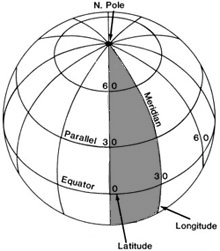
\includegraphics[scale = 4]{latlon.jpg}
\end{center}
\caption{An example of subset in grey}
\end{figure}

We classified the data according to the latitude, creating five classes listed in the table below. A more visual picture of our classification is given when we introduce the results of the different dimension reduction methods. The latitudes we chose are universally know parallels. The north temperate zone extends from the tropic of cancer to the arctic circle and the south temperate zone from the tropic of capricorne to the antarctic circle. 

\begin{figure}[H]
 \begin{center}
	
	\begin{tabular}{|c|c|c|c|c|c|}
		 \hline    
	  	& North &Temperate North & Equator &  Temperate South & South\\ 
		\hline
		Latitudes & 90 to 66 & 66 to 23 & 23 to -23 & -23 to -66 & -66 to -90 \\
		\hline
		 & \tikz\draw[blue,fill=blue] (0,0) circle (.5ex); & \tikz\draw[red,fill=red] (0,0) circle (.5ex); & \tikz\draw[green,fill=green] (0,0) circle (.5ex); & \tikz\draw[yellow,fill=yellow] (0,0) circle (.5ex); & \tikz\draw[pink,fill=pink] (0,0) circle (.5ex); \\
		\hline
		\% of Earth surface & 4 & 26 & 40 & 26 & 4 \\
		\hline
		  \end{tabular}
\end{center}
\caption{Our classification  }
\end{figure}

\section{Methods}

In all dimension reduction techniques, the main goal is to figure out a similarity function between vectors. Such a function will then enable to sort the dataset into classes of vectors with similar features, which would have been more intricate with the initial dataset. 

Our project was two sided. First, we familiarized with various dimension reduction techniques, then we attempted to show that the geographical position of a point on the planet - e.g. it's latitude and longitude - were embedded in the climate data one could gather on it. 

	\subsection{Principal Component Analysis - PCA}
	
		Principal Component Analysis detects tendencies in the data by maximizing the variance of the dataset matrix. There is an easy approach to understand PCA with a 2D dataset. On Figure \ref{4}, we can see the plot of a 2D-dataset. If we implement 2D-PCA, we will find two new axes that reflect at best the covariance of the samples. Those ares the green axes. PCA just rotates the figure to find a more explicit "point of view". The yielded axes are a linear combination of the original axes. 
		
		\begin{figure}[H]
 \begin{center}
	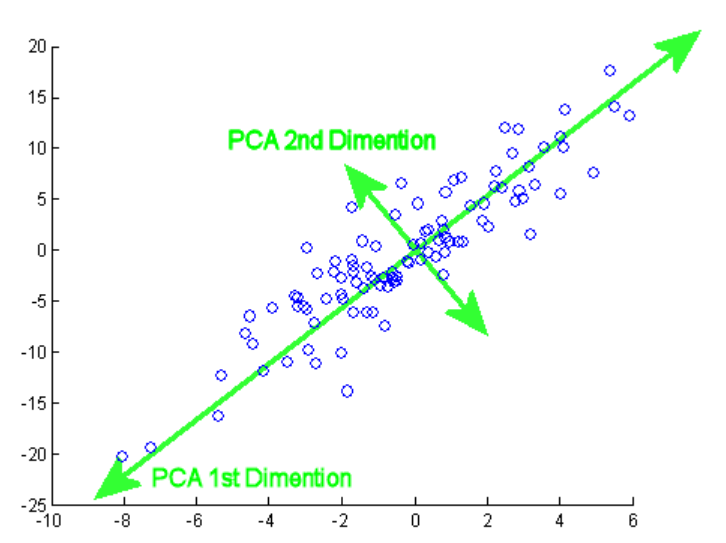
\includegraphics[scale = 0.5]{PCAexpli.png}
\end{center}
\caption{role of PCA  - interpretation}
\label{4}
\end{figure}
		
		
		From a mathematical point of view, PCA yields an orthonormal matrix that can be diagonalized. The largest eigenvalues point to the eigenvectors that contain the most information about the dataset. The dataset can then be projected on a lower dimension using the right eigenvectors.
		
		Let $ X \in \mathbb{R}^{d \times n} $ be our dataset where d is the number of variables and n the sample size, PCA maximizes the following equation :
%%
\[ \| X - MM^{T}X \|^{2}_{F} \]
subject to $ M \in \mathcal{O}^{d \times r} $ where $ r<d $ and $ \mathcal{O}^{d \times r}  $ is the space of orthonormal matrix and we use the Froebenius norm.

The maximum of the previous function is reached by the covariance matrix of the dataset: the r greatest eigenvalues of $ XX^{T} = PDP^{T}$ yield the maximum $ M = P_{r} $ where the columns are the eigenvectors associated to the eigenvalues mentioned above. The largest eigenvalues point to the eigenvectors that contain the most information about the dataset. 

The new dataset is thus $ Y = P_{r}^{T}X $ of dimensions $ r \times n $. In this example, there are r principal components for the PCA. Each of the $ M_{ij} $ coefficients of the matrix can be interpreted as weights given to the variable they are associated to. This enables us to interpret which variable of the dataset gives more significant information about the data. 

	\subsection{Kernel PCA}

Kernel Principal Component analysis is a non linear method for dimension reduction. Instead of directly maximizing the variance of $X$, we map it into a larger dimension space called the feature space, using a non linear function $\phi : \mathbb{R}^{d} \rightarrow \mathbb{R}^{N} $ where $N>d$. 
	
	Instead of directly mapping $X$ into the feature space, we use a kernel, that represents a similarity function between pairs. Let $K: \mathbb{R}^{d} \times \mathbb{R}^{d} \rightarrow \mathbb{R} $ be this kernel, then 
	\[ K(x_{i},x_{j}) = \phi(x_{�})^{T} \phi(x_{j})\]
where $(x_{i}, x_{j} ) \in \mathbb{R}^{d} \times \mathbb{R}^{d} $�are vectors of the dataset $X$ 
	
	This kernel will enable us to bypass the higher dimension calculation of the variance in the feature space. We only need to compute the pairwise values for $\phi$, but there is no need to explicitly define $\phi$.
	
	The downside of this method is that since we don't compute directly the eigenvectors and eigenvalues of $\phi$, the result is the projection of our dataset onto the eigenvectors. We thus don't have access to a simple interpretation of the principal components. 
	
	A classic kernel that is often used is the RBF function that is defined below: 
	 \[ K(x_{i},x_{j}) = e^{- \gamma \| x_{i} - x_{j} \| }\]
	
	\subsection{Multidimensional scaling}
	
	Multidimensional scaling is a linear approach to reduce dimension of a dataset. The principle is quite different from PCA: given a matrix of distance or "dissimilarity", MDS aims at reconstructing a map preserving at best the distances between datas. In our example, the MDS algorithm aims to place each object in a 2-dimensional space such that the between-object distances are preserved as well as possible.
	Given a distance matrix D of dimension $ n \times p $ (p=5 for us) , MDS attempts to find the datapoints $y_1$,... $y_t$ in dimension $d<p $(d=2 for us) that minimizes:
	
		 \[\sum\limits_{i=1}^{t}[\sum\limits_{j=1}^{t}d_{ij}^{(X)}-d_{ij}^{(Y)}]
			\]
		
	with $d_{ij}^{(X)}$ the euclidean distance between pairwise i and j in the original  $n \times p$ matrix $D^{(X)}$ and $d_{ij}^{(Y)}$ the euclidean distance between pairwise i and j in the original  $n \times p$ matrix $D^{(X)}$  and in the computed $ n \times d $ matrix $D^{(Y)}$.
	
	A basic approach to understand MDS is to use the example of cities. The input is the distance matrix between cities on the left on figure \ref{5}. MDS enables us to find the coordinates of each city based on this distance matrix.
	
	\begin{figure}[H]
 \begin{center}
	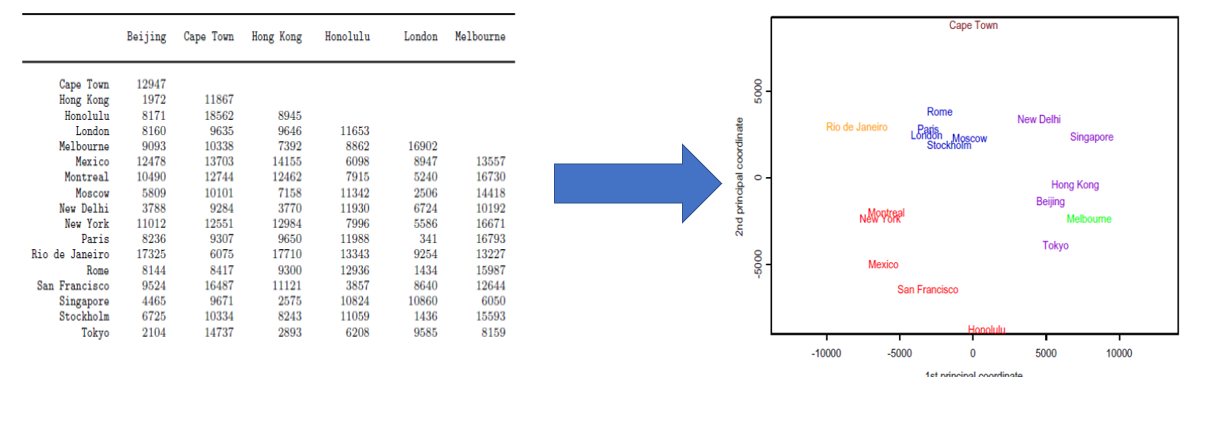
\includegraphics[scale = 0.4]{MDSexpli.png}
\end{center}
\caption{role of MDS  - interpretation}
\label{5}
\end{figure}

	\subsection{Isomap}
	
	Isomap is a low dimensional embedding method similar to MDS. The difference is that distance is not computed with euclidean norm but with geodesic distance. As the earth shape is round, isomap seems more relevant than MDS. On figure \ref{6}, we can see the difference between the geodisic distance (in red) used in isomap, and the eucliean distance used in MDS (in blue).
	
	\begin{figure}[H]
 \begin{center}
	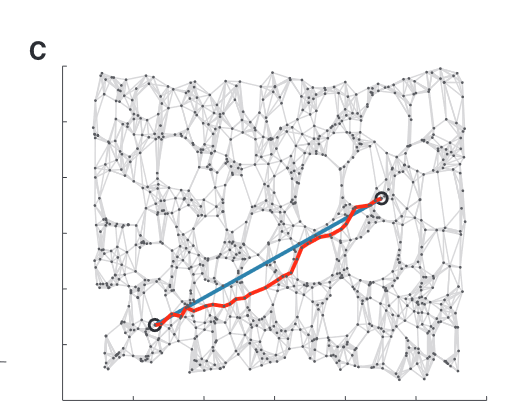
\includegraphics[scale = 0.6]{isoexpli.png}
\end{center}
\caption{geodisic and euclidean distance}
\label{6}
\end{figure}
	

\section{Results}
	\subsection{Graphic Interpretation}
		\subsubsection{PCA}
		
		We first implemented PCA and ran it with only two principal components, which yielded the graph plotted in figure \ref{7} for the whole dataset. We wrote the eigenvectors $ y_{1}�$ and $ y_{2}$ that were used horizontally to make it easier to understand their meaning. 
		
\begin{center}
	\begin{tabular}{ccccc}
		 \hline    
		 Temperature & Pressure&  Relative Humidity& Wind Speed& Radiation\\ 
		\hline
		  \end{tabular}
\bigskip
		
		$ y_{1} = [\,-0.94 \quad -0.31\quad 0.11 \quad -0.04 \quad 0.01\,] $

\bigskip
		$ y_{2} = [\,  0.03 \quad  -0.40 \quad -0.91 \quad 0.04 \quad -0.05\,] $
\end{center}
		
		This enables us to understand the meaning of these vectors. $ y_{1} $ is mostly related to a decreasing temperature and pressure, and $ y_{2} $ represents decreasing humidity and pressure. 

\begin{figure}[H]
	\centering
	\begin{minipage}[r]{.66\linewidth}
      		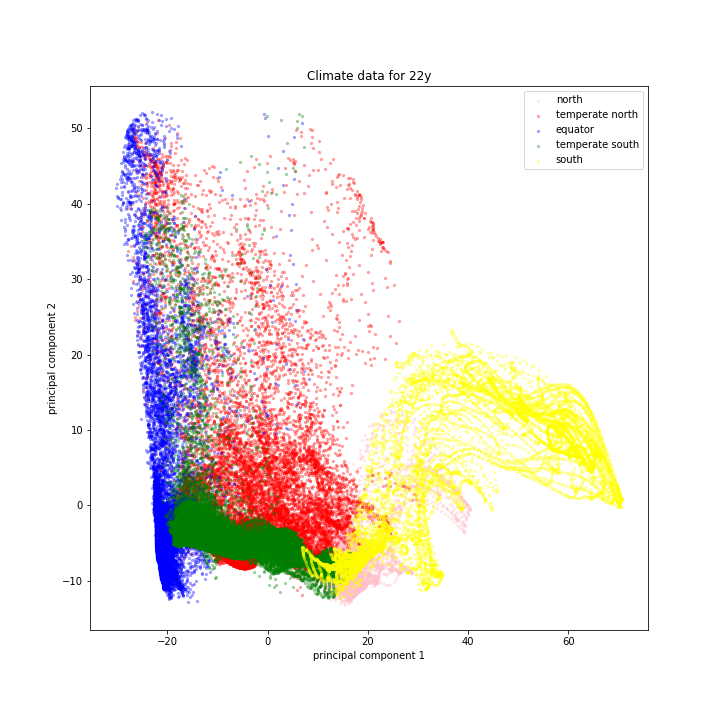
\includegraphics[scale=0.5]{pca2.png} %gauche bas droite haut
        \end{minipage}
         \hfill%
         \begin{minipage}[l]{.22\linewidth}
        		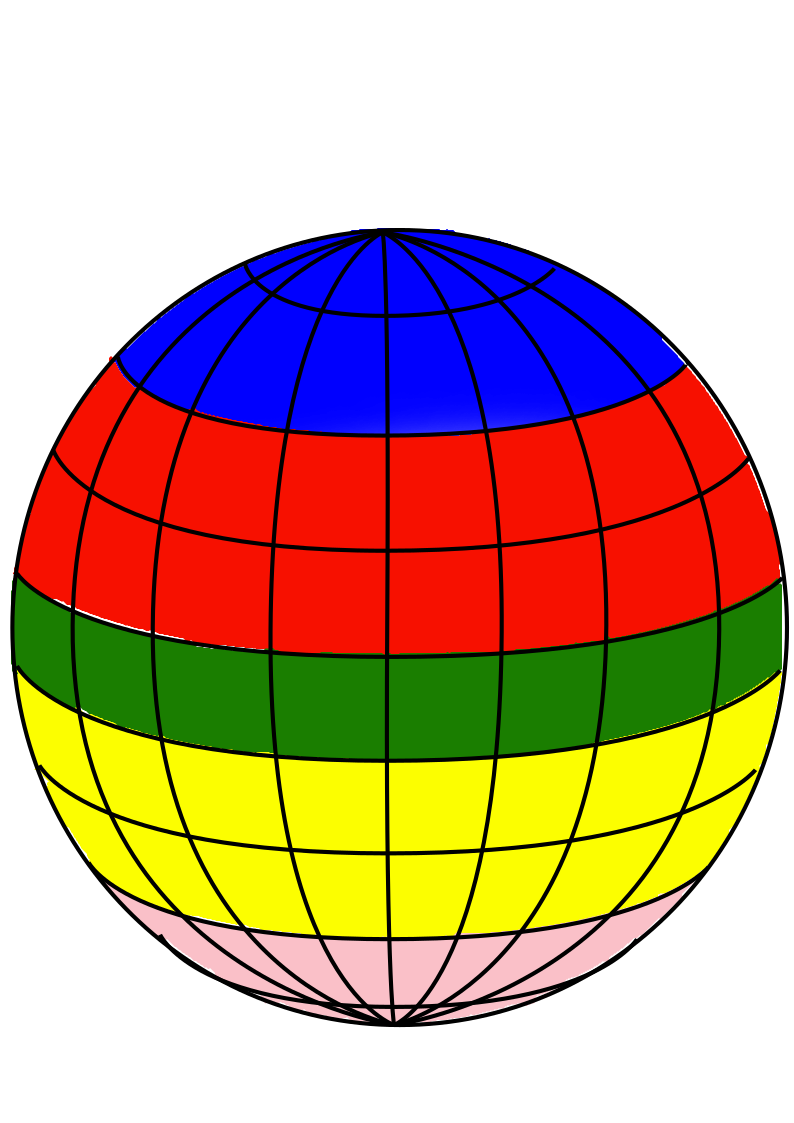
\includegraphics[scale=0.15]{colors.png}
    \end{minipage}
    \caption{PCA with two components}
    \label{7}
\end{figure}	

 \begin{center}
	\begin{tabular}{|c|c|c|c|c|}
		 \hline    
	  	 North &Temperate north & Equator &  Temperate South & South\\ 
		\hline
		  \tikz\draw[blue,fill=blue] (0,0) circle (.5ex); & \tikz\draw[red,fill=red] (0,0) circle (.5ex); & \tikz\draw[green,fill=green] (0,0) circle (.5ex); & \tikz\draw[yellow,fill=yellow] (0,0) circle (.5ex); & \tikz\draw[pink,fill=pink] (0,0) circle (.5ex); \\
		\hline
		  \end{tabular}
\end{center}

We can see on the graph that even if there is a strong dispersion, equator values are located at higher temperatures. On the contrary, north and south pole values are located at lower temperatures. Green and red classes overlap as these to categories have similar climate conditions. 

Although it is an understandable figure, this is not satisfying. 

		\subsubsection{Three dimensions}
		
We attempted to run the PCA method with three principal components, it yielded similar results as linear PCA, but some areas with particular climate conditions stood out more strikingly. For example, deserts are located at the bottom of the peak on the third figure below, that maps the dry and hot areas. 
		
\begin{figure}[H]
	\centering
	\begin{minipage}[c]{.30\linewidth}
       		 \centering
      		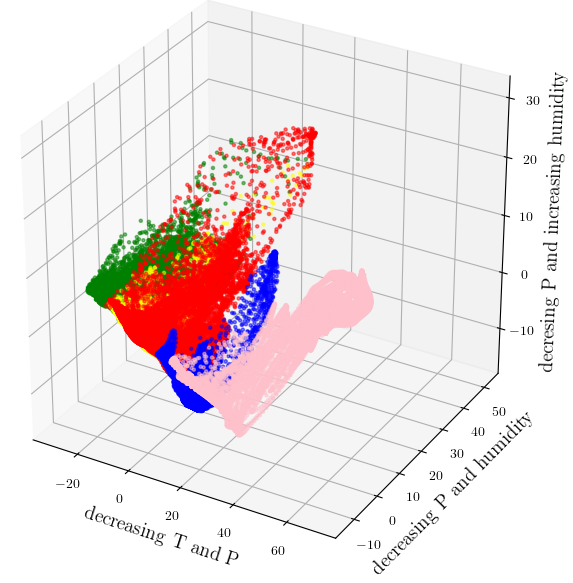
\includegraphics[scale=0.25]{3Dpca1.png} %gauche bas droite haut
		\centering
        \end{minipage}
         \hfill%
         \begin{minipage}[c]{.30\linewidth}
                  \centering
        		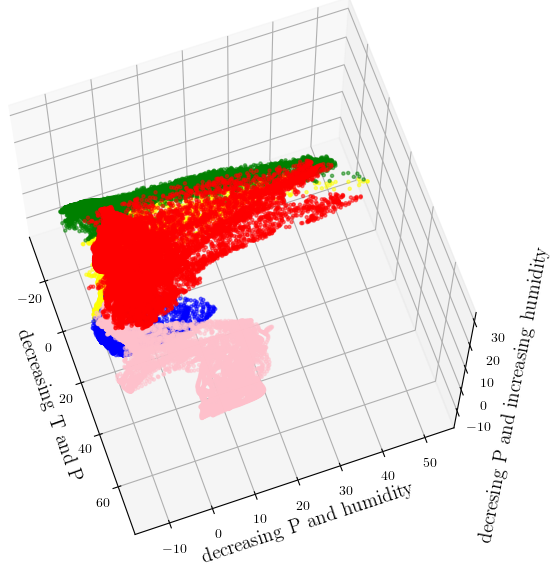
\includegraphics[scale=0.25]{3Dpca2.png}
        		\centering
    \end{minipage}
     \begin{minipage}[c]{.30\linewidth}
                  \centering
        		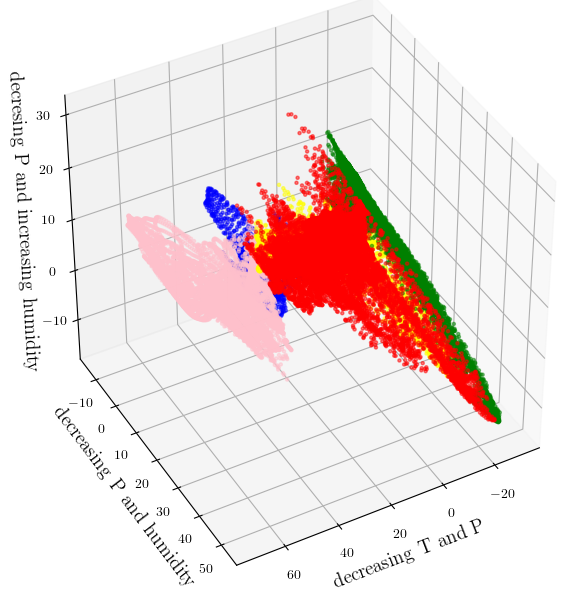
\includegraphics[scale=0.25]{3Dpca3.png}
        		\centering
    \end{minipage}
    \caption{3D PCA  }
\end{figure}

		
		
			\subsubsection{Kernel PCA}
	
	Kernel PCA has a complexity of $ O(n^{3}) $ so we decided to run it on a subset of our dataset. Here is the two dimension result for all latitudes between longitudes -15 and +15. 

\begin{figure}[H]
	\centering
	\begin{minipage}[c]{.66\linewidth}
       		 \centering
      		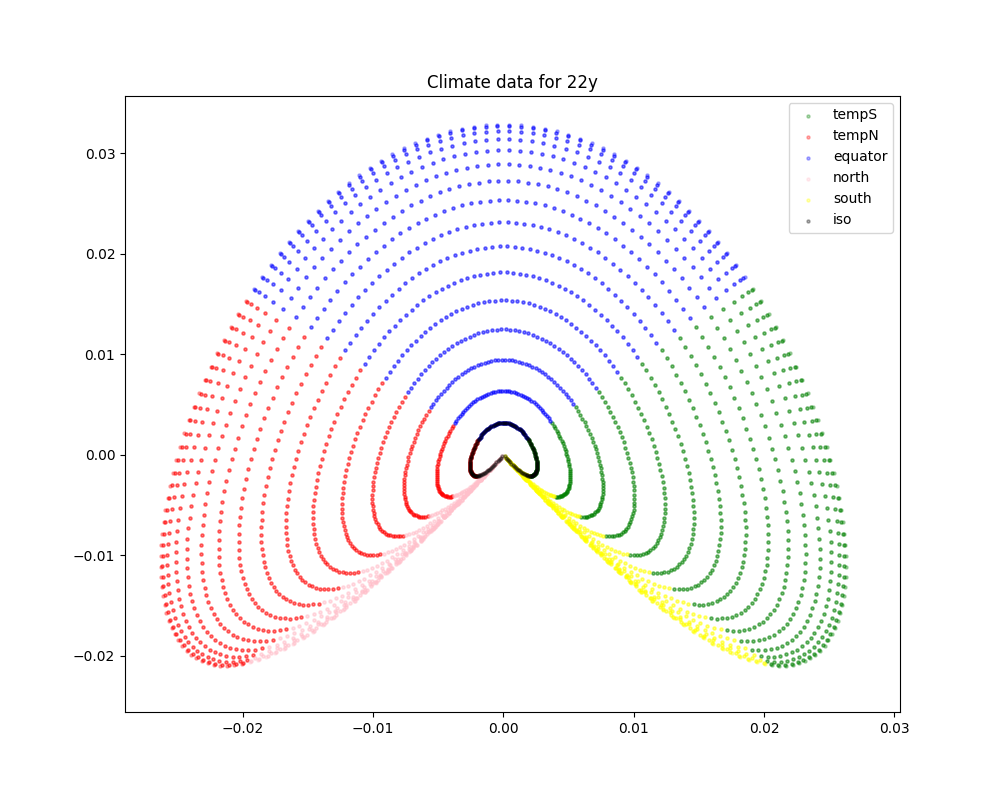
\includegraphics[scale=0.5]{kpca_first.png} %gauche bas droite haut
		\centering
        \end{minipage}
         \hfill%
         \begin{minipage}[c]{.26\linewidth}
                  \centering
        		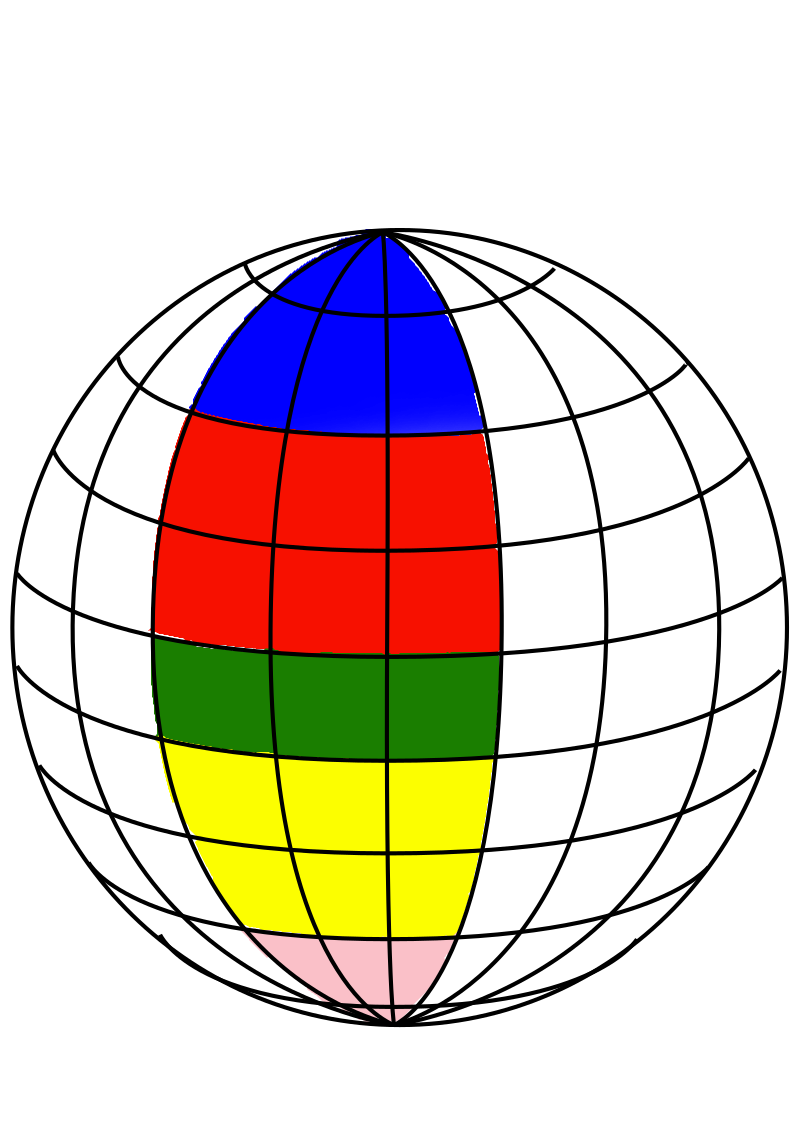
\includegraphics[scale=0.2]{colorslice.png}
        		\centering
		
    \end{minipage}
    \caption{Kernel PCA with two components and the RBF kernel}
\end{figure}

	The black dots are all dots along one longitude, here 15. We see however that there is a degenerescence: -15 and +15 longitude are projected on the same positions. When changing the $ \gamma $, some lines grow appart but most of them stay degenerated.
	Another flow of this representation is the space that is taken by the equator area. When representing the temperature in this area, we can see it does not vary very much compared to other regions: the variables should be represented closer together, as it was the case for example in PCA. 
	
	The peak present in the center of the figure is a consequence of the fact that data from each side of the peak even if they are close numerically are not close spatially: they are the data from both north and south pole. 
	
\begin{figure}[H]
	\centering
	\begin{minipage}[c]{.30\linewidth}
       		 \centering
      		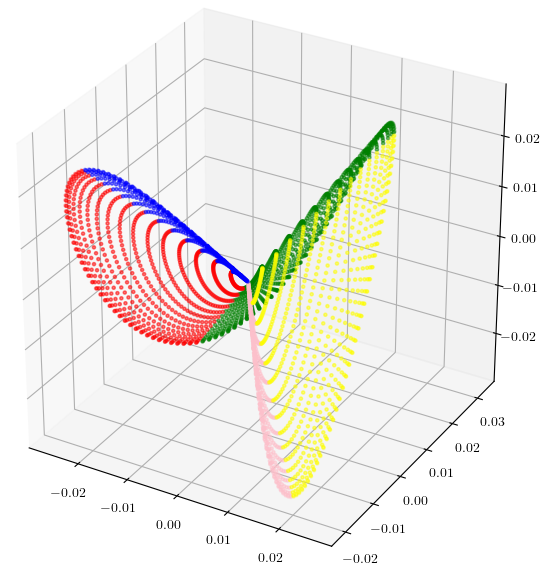
\includegraphics[scale=0.3]{3Dkpca1.png} %gauche bas droite haut
		\centering
        \end{minipage}
         \hfill%
         \begin{minipage}[c]{.30\linewidth}
                  \centering
        		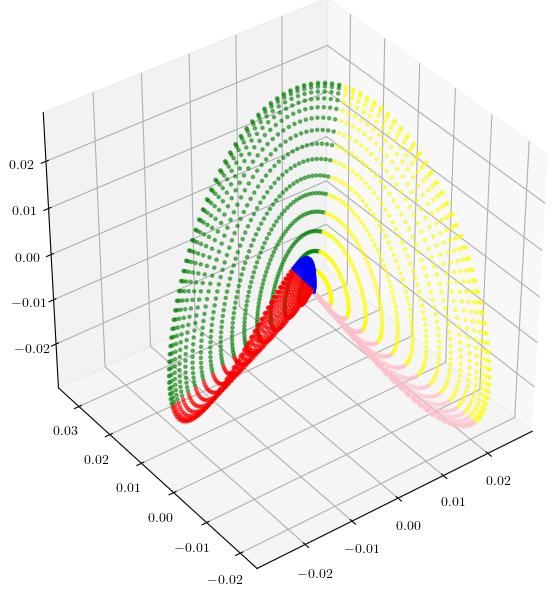
\includegraphics[scale=0.3]{3Dkpca2.png}
        		\centering
    \end{minipage}
     \begin{minipage}[c]{.30\linewidth}
                  \centering
        		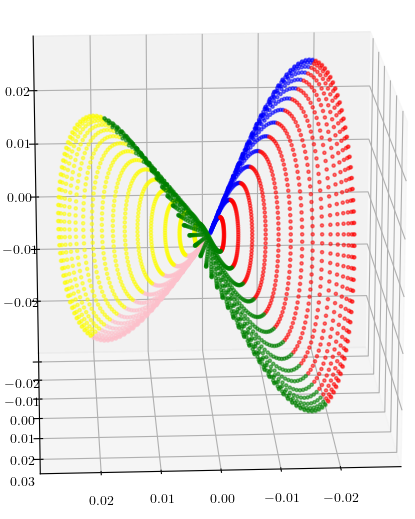
\includegraphics[scale=0.3]{3Dkpca3.png}
        		\centering
    \end{minipage}
    \caption{3D Kernel PCA}
    \end{figure}	


The dots representing the south and north poles are still closer together however, which might come from the smaller range of temperatures and climate conditions reached in these areas. 

 Changing the kernel function to a polynomial one however destroyed the degenerescence, but created a node on equatorial values as it can be observed just below. The purple and black lines represent the -15 and 15 longitudes: they are clearly different. 

\begin{figure}[H]
	\centering
	\begin{minipage}[c]{.66\linewidth}
       		 \centering
      		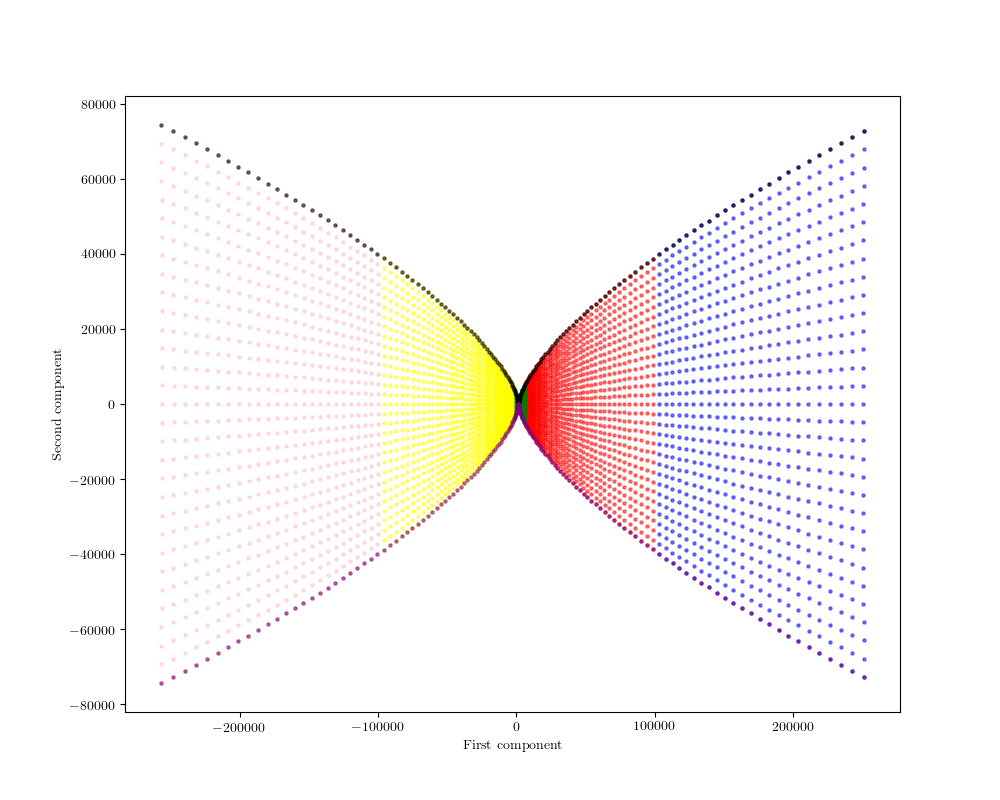
\includegraphics[scale=0.5]{kpca_poly.png} %gauche bas droite haut
		\centering
        \end{minipage}
         \hfill%
         \begin{minipage}[c]{.26\linewidth}
                  \centering
        		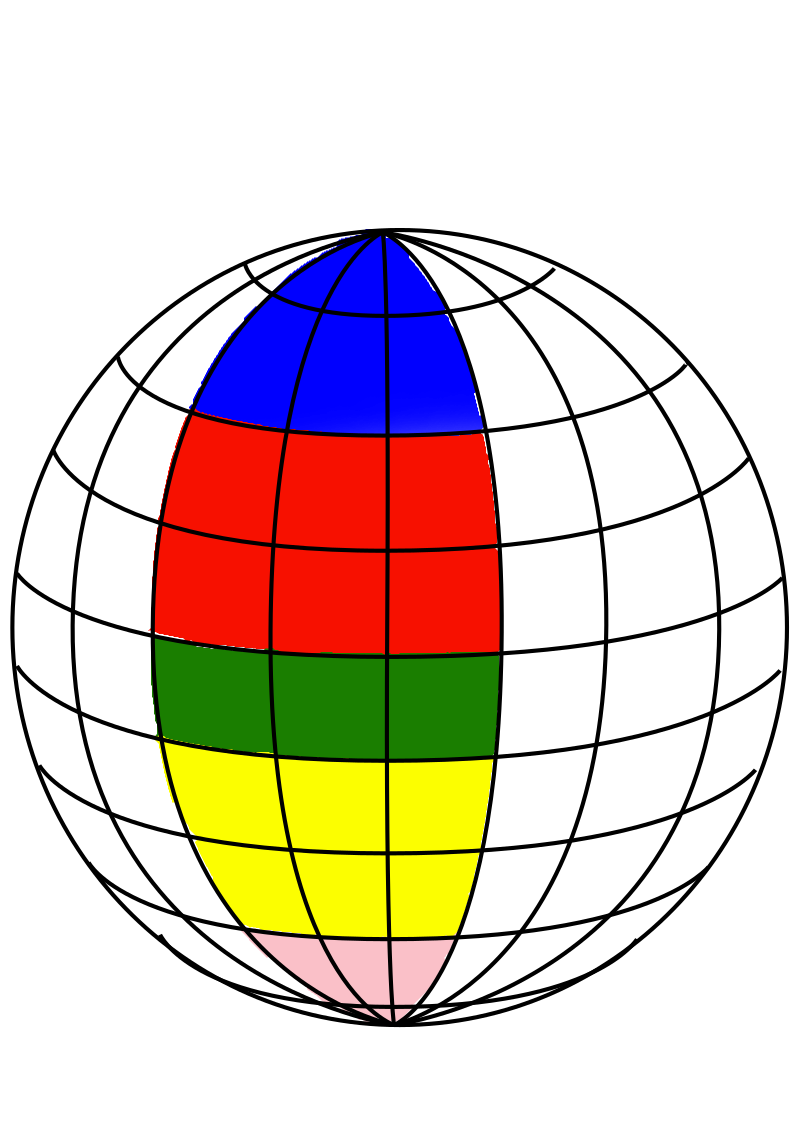
\includegraphics[scale=0.2]{colorslice.png}
        		\centering
		
    \end{minipage}
    \caption{Kernel PCA with two components and polynomial kernel}
\end{figure}

			\subsubsection{Multidimensional Scaling - MDS}
	
	As MDS was extremeley low and seemed to use a lot of memory, we could not run the programm for more than 600 datapoints (ie 600 rows).Therefore, we used a new subset of longitudes between 0� and +5�, reducing the dataset size to 546 datapoints. 
	Figure 6 shows the results of MDS. As we can see, datas from South pole and North pole are quite compact, that is to say that all points are near each other. There is not a wide range of temperature, pressure, radiation, humidity and wind speed in those regions. This is quite what we expected. 
	On the contrary, regions like equator and north temperate show a wide range of climatic parameters as some points are quite far from each other. It would mean that there are more diverse climate in equator and north temperate. It also seems like south temperate shows less diversity of climate as all the points seem compact. This is not what we expected, as south and north temperate are supposed to have same characteristics. This could be explained by two reasons. \textbf{Either we are missing information because we have reduced too much the dimension, or south hemisphere is quite different because it has much more ocean than the north hemisphere.} To check the first possibility, we implemented MDS in 3D, here are the results on figure ??. As we can see, the yellow points (south temperate) are not as widely spread as the green (equator) or red (north temperate) one. So it seems like the second possibility explain why we have fewer variance of climatic parameters in south temperate.
	
	\begin{figure}[H]
 \begin{center}
	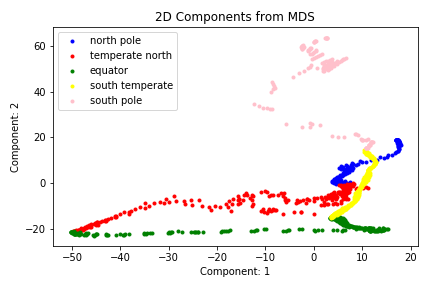
\includegraphics[scale = 0.7]{graphMDS.png}
\end{center}
\caption{Results of MDS in 2D}
\end{figure}

\begin{figure}[H]
 \begin{center}
	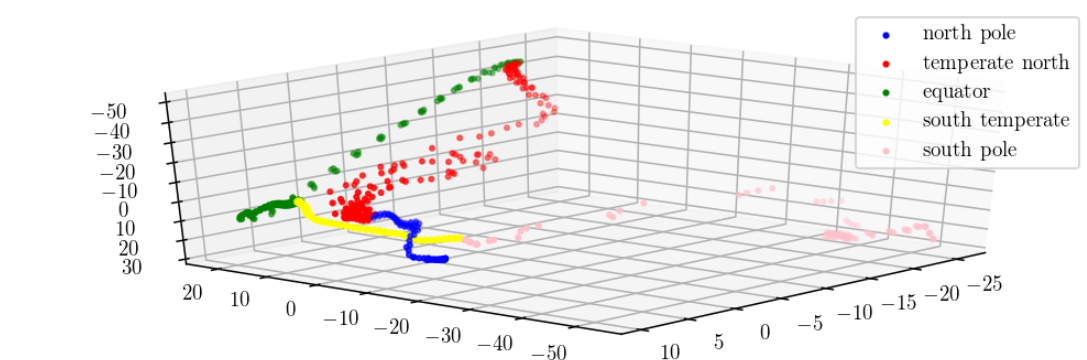
\includegraphics[scale = 0.5]{mds3Da.png}
\end{center}
\caption{Results of MDS in 3D}
\end{figure}

\begin{figure}[H]
 \begin{center}
	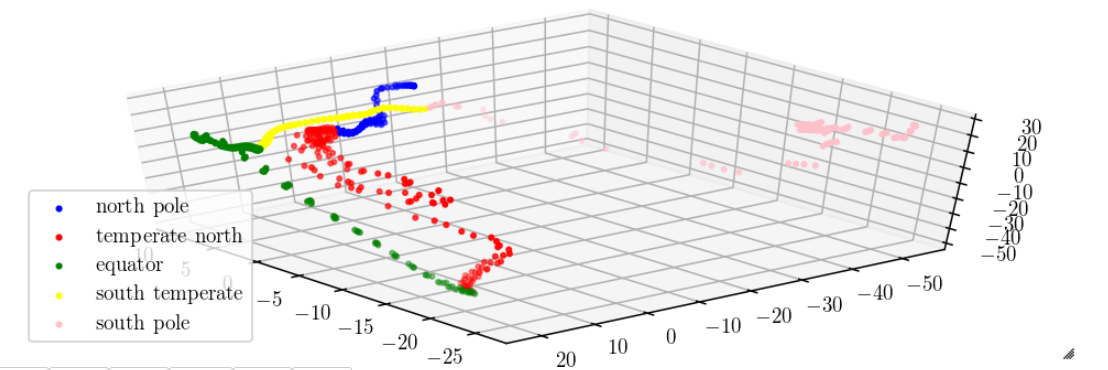
\includegraphics[scale = 0.5]{mds3Db.png}
\end{center}
\caption{Results of MDS in 3D}
\end{figure}

 
			\subsubsection{Isomap}
	
	One of the key parameter of isomap  is the number of nearest neighbors taken into account. Therefore, we present in figure  ?? the result of isomap for number of neighbour between 1 to and neighbors. 
	
	\begin{figure}[H]
 \begin{center}
	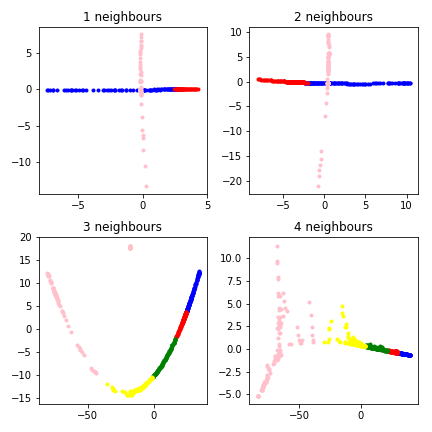
\includegraphics[scale = 0.8]{graphiso.png}
\end{center}
\caption{results of isomap depending on the number of neighbors considered from 2 to 8}
\end{figure}

It is obvious that the number of neighbours considered strongly influence the 2D distribution of our dataset. To know which graph is the most accurate, we refer to the 'reconstruction error'. This reconstruction error is a function embedded in scikit. For the moment, we only need to know that it is an indicator of how much isomap mapping is accurate and respect original distance, it kind of computes difference between the final distance of two items in the isomap mappingl and the true distance between them. We computed this reconstruction error with respect to the number of neighbours considered. The results are presented in figure ??

\begin{figure}[H]
 \begin{center}
	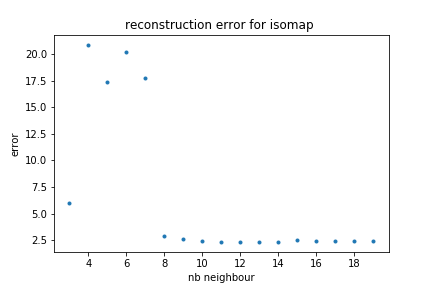
\includegraphics[scale = 0.8]{isoerrorneighbour.png}
\end{center}
\caption{reconstruction error as a function of number of neighbours considered}
\end{figure}

It is interesting to see that from eight neighbors, error seems to stabilize around 2,5. So the most 'accurate' representation should be with 8 neighbors. If we interpret the graph with 8 neighbors, we can see that we can browse the entire planet from north pole to south pole, going through all zones in the order, \textbf{which is not the case in MDS}. So isomap better preserve the geometry of the dataset. It is interesting to see that pink points(ie south pole) are much more spread in isomap than MDS.

\subsection{Time comparison}
	
	We implemented manually PCA, but for the other methods we used the built in fonction of the scikit package on python. 
	PCA's running time varies linearly with the dataset size as we can see on the graphic below 

\begin{figure}[H]
 \begin{center}
	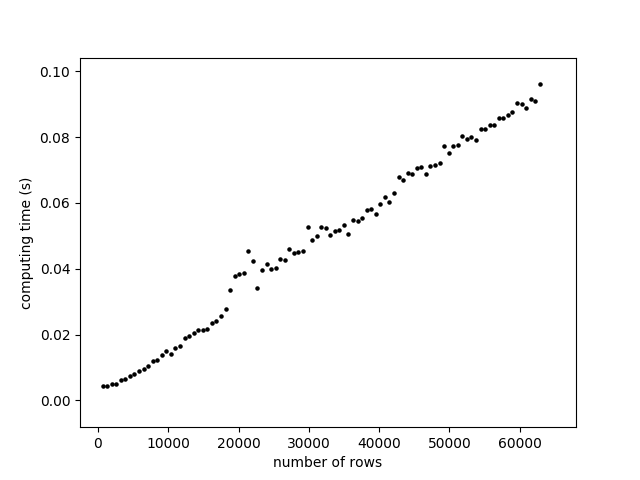
\includegraphics[scale = 0.5]{pcatime.png}
\end{center}
\caption{running time for PCA}
\end{figure}

Kernel PCA was slower, we did not compute its running time for all the dataset, only until 12000 rows. It yields the following graph. 

\begin{figure}[H]
	\centering
	\begin{minipage}[c]{.46\linewidth}
       		 \centering
      		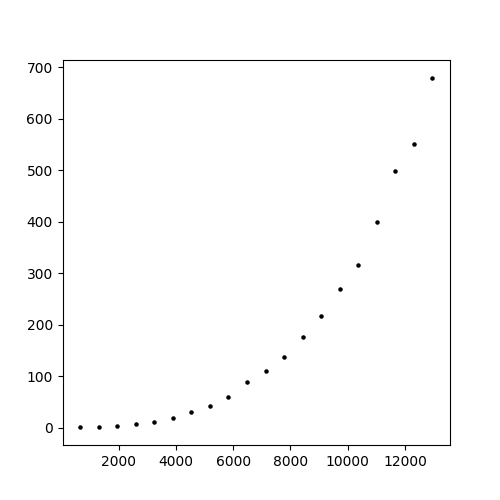
\includegraphics[scale=0.5]{kpcatime.png} %gauche bas droite haut
		\centering
		\caption{running time for Kernel PCA}
        \end{minipage}
         \hfill%
         \begin{minipage}[c]{.46\linewidth}
                  \centering
        		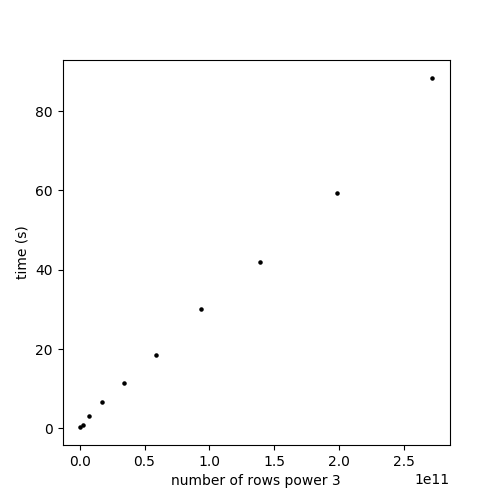
\includegraphics[scale=0.5]{kpcatimpe.png}
        		\centering
		\caption{Kernel PCA running time is a $O(n^{3})$}
    \end{minipage}
\end{figure}

	In figure 10, we present computing time for the four different methods as a function of the sample size.
	From this we can conclude that the quickest method is PCA. Then come isomap, kernel PCA and finally MDS. It is quite surprising to see that isomap is quicker than MDS for the same number of rows. Indeed, isomap uses the same algorithm than MDS but also needs to compute distance with neighbors first. It is thus expected to be slower. We found an explanation on the 'manifold guide' of skicit.
	
	\begin{quotation}
\begin{quote}
In Scikit-Learn implementation, Isomap algorithm runs faster that Multi Dimensional Scaling on the S-Curve dataset [...]. In the third stage of algorithm, the implementation uses Partial Eigen Value decomposition instead of MDS which is the version proposed by the researchers	
	\end{quote}		
	\end{quotation}
	
	We did not use the 'S curve dataset' as mentioned above, but we may think that due to the round shape of earth, our dataset is quite similar to the S-curve and thus Isomap runs faster than MDS. For a fixed dimension d, the following table present the complexity of every method as it appeared to us.

\bigskip
 \begin{center}
		\begin{tabular}{|c|c|c|c|c|}
		 \hline    
	  	Method & PCA & Kernel PCA & MDS & Isomap \\ 
		\hline
		Complexity & $O(nr^{2})$ & $O(n^3)$ & $O(n^3)$  &  \\
		\hline
		  \end{tabular}
 \end{center}

\begin{figure}[H]
 \begin{center}
	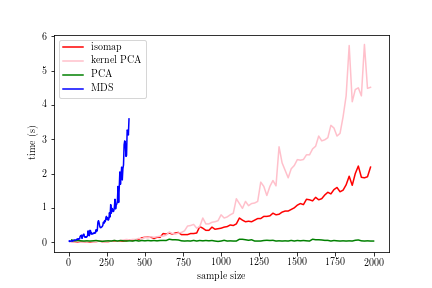
\includegraphics[scale = 0.8]{time.png}
\end{center}
\caption{computing time comparison}
\end{figure}


We also check how isomap computing time varies with the number of neighbor taken into account. Figure 11 shows that isomap efficiency time increases with the number of neighbors. So isomap efficiency of computing time may be limited by the number of neighbors.

\begin{figure}[H]
 \begin{center}
	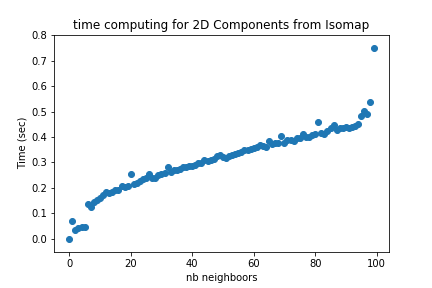
\includegraphics[scale = 0.8]{timeisoneigh.png}
\end{center}
\caption{computing time for isomap as a function of the number of neighbors considered}
\end{figure}

\subsection{Error and preserved information}
\subsubsection{PCA}

	The main indicator of how much information has been preserved with PCA lies in eigenvalues. We plot the eigenvalues to see their relative importance in the dimension reduction.

\begin{figure}[H]
 \begin{center}
	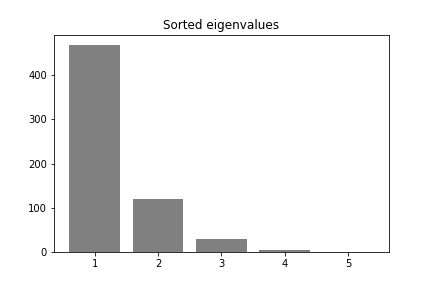
\includegraphics[scale = 0.6]{eigen.png}
\end{center}
\caption{PCA with two components}
\end{figure}

We can see that with only two components, we obtain an explained variance of 94\%, which is quite enough to interpret our dataset. PCA seems to be a relevant technic to analyse data, and in particular to establish classification.
		
We also reconstructed the dataset from its projection with PCA. It is indeed possible to build an estimated $ \hat{X} $ dataset from the projected data of PCA. We plotted the first column of the dataset, the temperature for $X $ and $ \hat{X} $ as a function of latitude and longitude. Even if the curve is reversed and the numerical values are not correct, the structure of the data is saved. 
		
\begin{figure}[H]
	\centering
	\begin{minipage}[c]{.30\linewidth}
       		 \centering
      		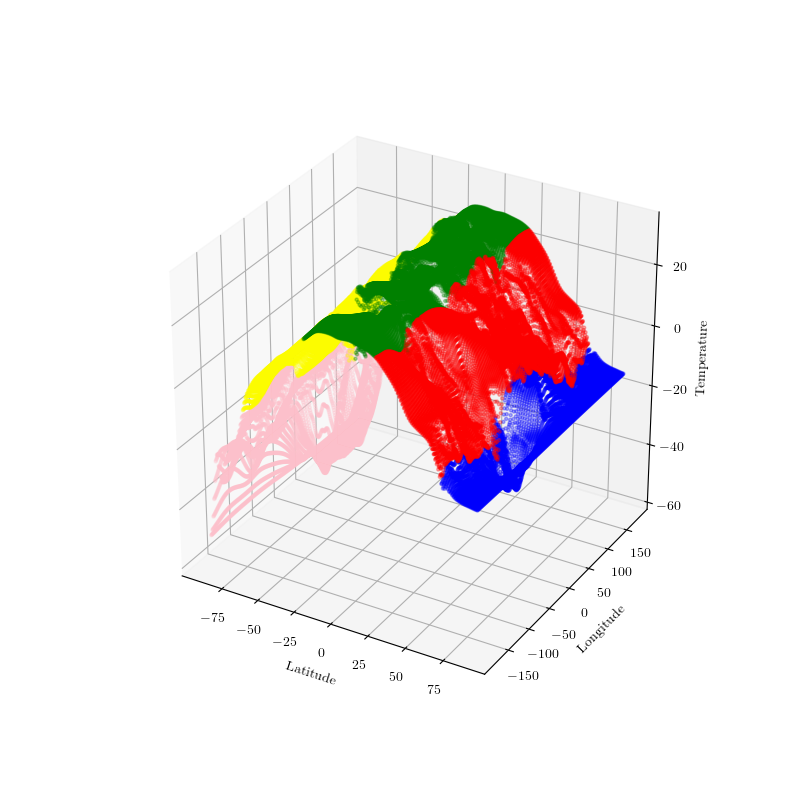
\includegraphics[scale=0.4]{temp1.png} %gauche bas droite haut
		\centering
        \end{minipage}
         \hfill%
         \begin{minipage}[c]{.30\linewidth}
                  \centering
        		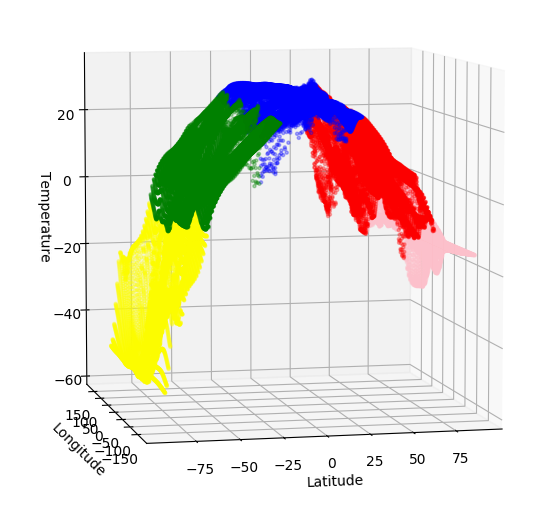
\includegraphics[scale=0.3]{temp2.png}
        		\centering
    \end{minipage}
     \begin{minipage}[c]{.30\linewidth}
                  \centering
        		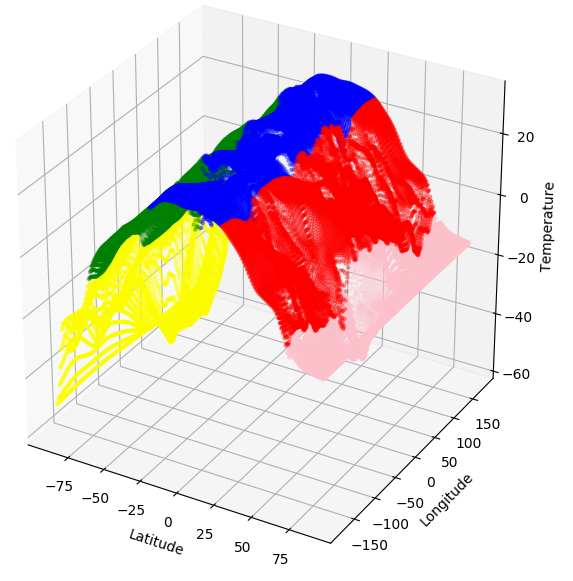
\includegraphics[scale=0.3]{temp3.png}
        		\centering
    \end{minipage}
    \caption{Temperature as a function of latitude and longitude in $X$ }
\end{figure}

\begin{figure}[H]
	\centering
	\begin{minipage}[c]{.30\linewidth}
       		 \centering
      		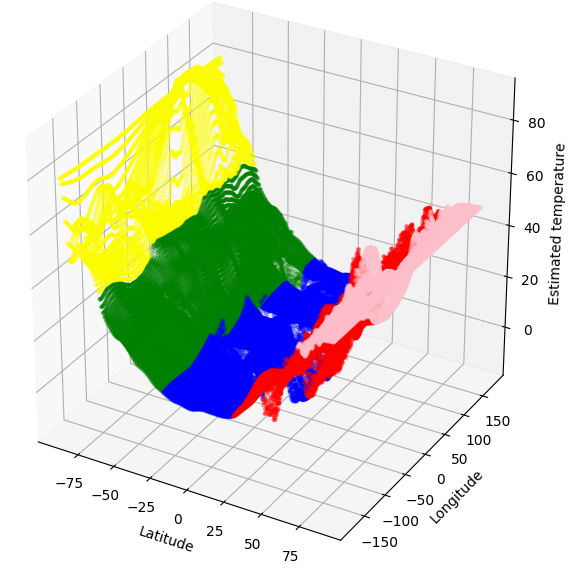
\includegraphics[scale=0.3]{esttemp1.png} %gauche bas droite haut
		\centering
        \end{minipage}
         \hfill%
         \begin{minipage}[c]{.30\linewidth}
                  \centering
        		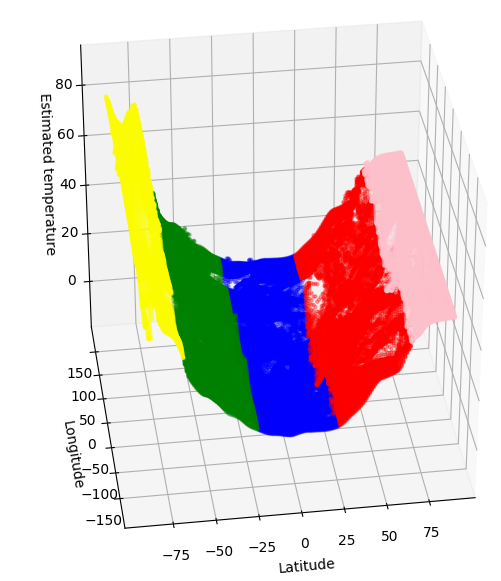
\includegraphics[scale=0.3]{esttemp2.png}
        		\centering
    \end{minipage}
     \begin{minipage}[c]{.30\linewidth}
                  \centering
        		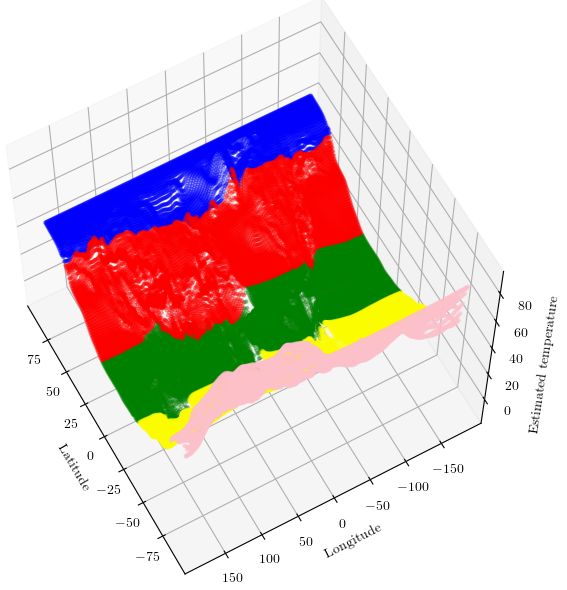
\includegraphics[scale=0.3]{esttemp3.png}
        		\centering
    \end{minipage}
    \caption{Temperature as a function of latitude and longitude in $\hat{X}$ }
\end{figure}


			\subsubsection{MDS and isomap}
			
			As isomap and MDS function with the same principle, we decided to compare their estimated error. For MDS, we ued an indicator called stress. It is roughly the square difference between the final distance of two items in the MDS model and the true distance between them. The exact formula is: 
		
			\[ s = \sqrt{\frac{\sum (d_{ij}-d(i,j))}{\sum d_{ij}}}
		\]
		
with $d_{ij}$ the original distance between pairwaise i and j and d(i,j) the computed distance. The aim of MDS is to minimize this stress.  For isomap, there is an indicator called error reconstruction already embedded in scikit. We will not detail its formula here as it is quite heavy and complicated. All we need to know is that it can be compared to the notion of stress as in MDS in the sense that it computes the difference between the final distance of two items in the MDS model and the true distance between them.
		
	\begin{figure}[H]
 \begin{center}
	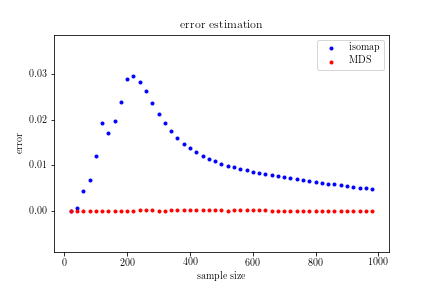
\includegraphics[scale = 1]{compmdsiso.png}
\end{center}
\caption{stress as a function of sample size}
\end{figure}

As we can see, isomap is less efficient than MDS for a subset of size 200. AS the data set size increases, isomap error tends to lessen but is still much more important than MDS error. \textbf{In our example, it seems like MDS gives a much more accurate representation of our dataset.}

	Then, we intended to see how reconstruction error evolve with the number of dimension taken into account for both MDS and isomap. On figure ?? we compare how reconstruction error evolve with dimension. We make dimension vary between 2 and 3.

\begin{figure}[H]
 \begin{center}
	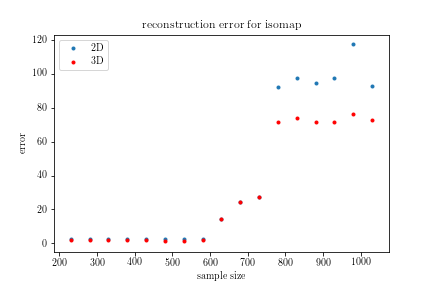
\includegraphics[scale = 0.8]{isoerrorsamplesizeD.png}
\end{center}
\caption{reconstruction error as a function of the sample size for ISOMAP}
\end{figure}

As the sample size increases, error for 2D isomap keep increasing compare to error in 3D isomap. As expected, error for 2D isomap is bigger than for 3D because we reduce more the dimension.

We did the same for MDS in 2D and 3D. 
		
\section{Conclusion}


\section{Bibliography}
\noindent
Datasets

\noindent
\label{dataset} https://eosweb.larc.nasa.gov/cgi-bin/sse/global.cgi?email=skip@larc.nasa.gov $\uparrow $[\pageref{url}]

\bigskip
\noindent
John P. CUNNINGHAM, Zoubin GHAHRAMANI, Linear Dimensionality Reduction: Survey, Insights, and Generalizations, , \textit{Journal of Machine Learning Research 16} (2015) 2859-2900

\bigskip
\noindent
Alon ORLITSKY, SAJAMA, Supervised dimensionality reduction using mixture models, Proceedings of the 22nd international conference on Machine learning, p.768-775, August 07-11, 2005, Bonn, Germany  

\end{document}